\renewcommand{\theequation}{\theenumi}
\begin{enumerate}[label=\thesection.\arabic*.,ref=\thesection.\theenumi]
\numberwithin{equation}{enumi}
\item 
Find the point at which the tangent to the curve 
%\cite{twelve_one}
\begin{align}
y = \sqrt{4x-3}-1
\label{eq:parab}
\end{align}
has slope $\frac{2}{3}$.
\\
\solution \eqref{eq:parab} can be expressed as
\begin{align}
\brak{y+1}^2 &= 4x-3
\\
\text{or, } y^2  -4x + 2y+ 4 &= 0
\label{eq:parab_twovar}
\end{align}
which has the form \eqref{eq:conic_quad_form} with parameters
\begin{align}
\vec{V} = \myvec{0 & 0\\0 & 1}, \vec{u} = \myvec{-2\\1}, f = 4.
\label{eq:parab_twovar_params}
\end{align}
Thus, the given curve is a parabola.  $\because \vec{V}$ is diagonal and in standard form,
\begin{align}
\vec{P} = \vec{I} \implies \vec{p}_1 = \myvec{1\\0}
\label{eq:parab_ex1_eig}
\end{align}
From Table \ref{table:conics}, the 
focus is 4
and the vertex $\vec{c}$ is
\begin{align}
\myvec{ -4 & 1 \\ 0 & 0 \\ 0 & 1}\vec{c} &= \myvec{-4 \\ 0\\-1} 
\\
\implies 
\myvec{ -4 & 1 \\  0 & 1}\vec{c} &= \myvec{-4 \\ -1} 
\\
\text{or, } \vec{c} = \myvec{\frac{3}{4}\\-1}
\end{align}
The direction vector and normal vectors are
\begin{align}
\vec{m} = \myvec{1 \\ \frac{2}{3}} = \myvec{3\\2}, \vec{n} = \myvec{2\\-3}.
\label{eq:parab_twovar_mn}
\end{align}
Also, 
\begin{align}
\vec{V}\vec{p} &= \vec{0}
\\
\implies \vec{p} &= \myvec{1\\0}
\label{eq:parab_twovar_p}
\end{align}
From \eqref{eq:conic_tangent_qk_eigen}, \eqref{eq:parab_twovar_mn} and \eqref{eq:parab_twovar_p},
\begin{align}
\kappa = -1
\end{align}
which, upon substitution in \eqref{eq:conic_tangent_q_eigen} and simplification yields the matrix equation
\begin{align}
\myvec{-4 & 4\\0 & 0\\0&1}\vec{q} &= \myvec{-4\\0\\2}
\\
\implies \myvec{-4 & 4\\0&1}\vec{q} &= \myvec{-4\\2}
\\
\text{or, } \vec{q} &= \myvec{3\\2}
\end{align}
Fig. \ref{fig:parab_tangent}	verifies the above results.
%
\begin{figure}[!ht]
\centering
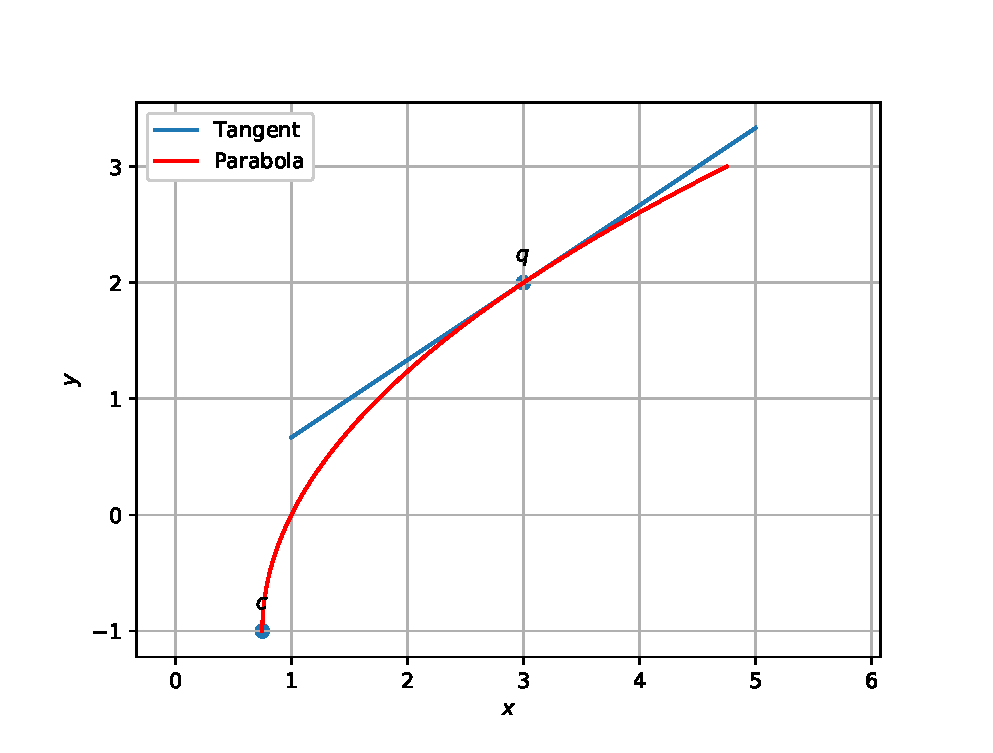
\includegraphics[width=\columnwidth]{./figs/parab/parab_tangent.eps}
\caption{Tangent to  parabola in \eqref{eq:parab}  with slope $\frac{2}{3}$. }
\label{fig:parab_tangent}	
\end{figure}

\item 
Find a point on the curve 
%\cite{twelve_one}
\begin{align}
y = \brak{x-2}^2
\label{eq:parab_secant}
\end{align}
at which the tangent is parallel to the chord joining the points (2, 0) and (4, 4).
\\
\solution \eqref{eq:parab_secant} can be expressed as
\begin{align}
x^2  -4x - y + 4 &= 0
\label{eq:parab_secant_twovar}
\end{align}
which has the form \eqref{eq:conic_quad_form} with parameters
\begin{align}
\vec{V} = \myvec{1 & 0\\0 & 0},  \vec{u} = -\myvec{2\\\frac{1}{2}}, f = 4.
\label{eq:parab_secant_twovar_params}
\end{align}
Using eigenvalue decomposition, 
\begin{align}
\vec{P} = \myvec{0 & 1\\1 & 0}, \vec{D} = \myvec{0 & 0\\0 & 1}
\end{align}
%
Hence, the eigenvector of $\vec{V}$ corresponding to the zero eigenvalue is
\begin{align}
\vec{p}_1 = \myvec{0\\1}.
\end{align}
Substituting the above parameters in the equation for the vertex of the parabola in Table \ref{table:conics},
\begin{align}
\myvec{-2 & -\frac{5}{2} \\ 1 & 0 \\ 0 & 0}\vec{c} &= \myvec{-4 \\ 2 \\ 0}
\\
\implies \myvec{-1 & -\frac{5}{2} \\ 1 & 0}\vec{c} &= \myvec{-4 \\ 2 }
\\
\text{or, } \vec{c} &= \myvec{2\\0}
\end{align}
The direction vector is
\begin{align}
\vec{m} = \myvec{4 \\ 4}-\myvec{2 \\ 0} = \myvec{1\\2}
\label{eq:parab_secant_twovar_m}
\end{align}
and normal vector is
\begin{align}
\vec{n} =  \myvec{2\\-1}
\label{eq:parab_secant_twovar_n}
\end{align}
From the equation for the point of contact for the  parabola  in Table \ref{table:conics},
%\eqref{eq:conic_tangent_qk_eigen}, \eqref{eq:parab_secant_twovar_params}
% and \eqref{eq:parab_secant_twovar_n} 
\begin{align}
\kappa = \frac{1}{2}
\end{align}
resulting in the matrix equation
\begin{align}
\myvec{-1 & -1\\1 & 0\\0&0}\vec{q} &= \myvec{-4\\3\\0}
\\
\implies \myvec{-1 & -1\\1 & 0}\vec{q} &= \myvec{-4\\3}
\\
\text{or, } \vec{q} &= \myvec{3\\1}
\end{align}
Fig. \ref{fig:parab_secant_tangent}	verifies the above results.  Note that $\vec{P}$ rotates the standard parabola by 90\degree.
%
\begin{figure}[!ht]
\centering
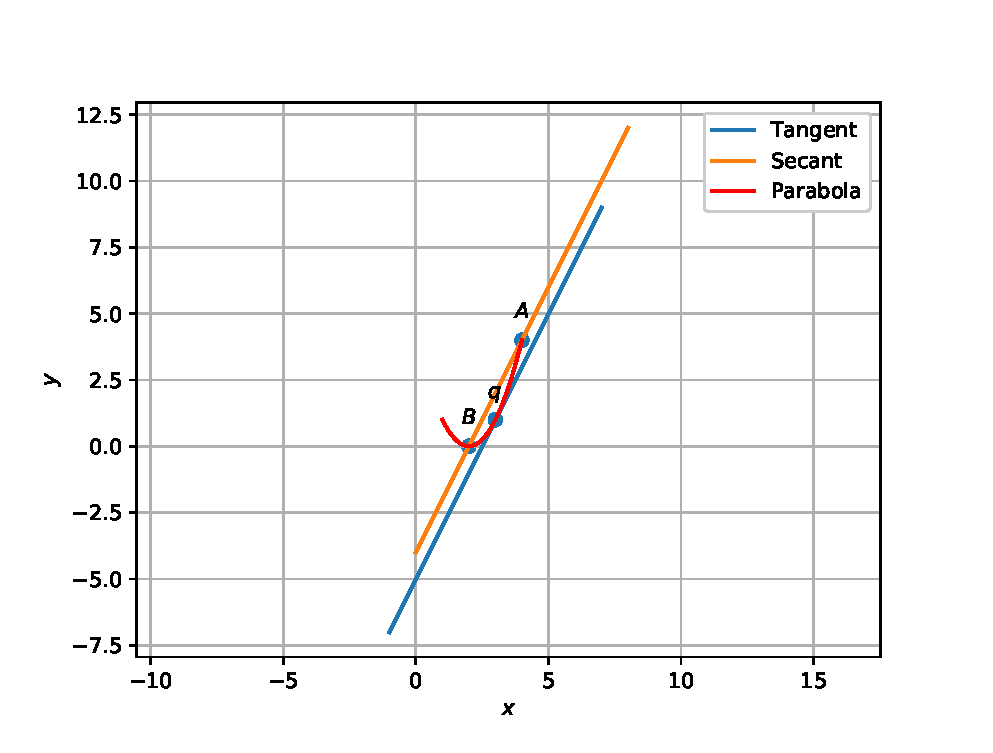
\includegraphics[width=\columnwidth]{./figs/parab/parab_tangent_secant.eps}
\caption{Tangent to  parabola in \eqref{eq:parab_secant}  is parallel to the line joining the points \myvec{2\\ 0} and \myvec{4\\ 4}. }
\label{fig:parab_secant_tangent}	
\end{figure}

\end{enumerate}
